\documentclass{standalone}
\usepackage{tikz}
\usepackage[utf8]{inputenc}
\usepackage[T1]{fontenc}
\usetikzlibrary{patterns,arrows.meta}

\begin{document}

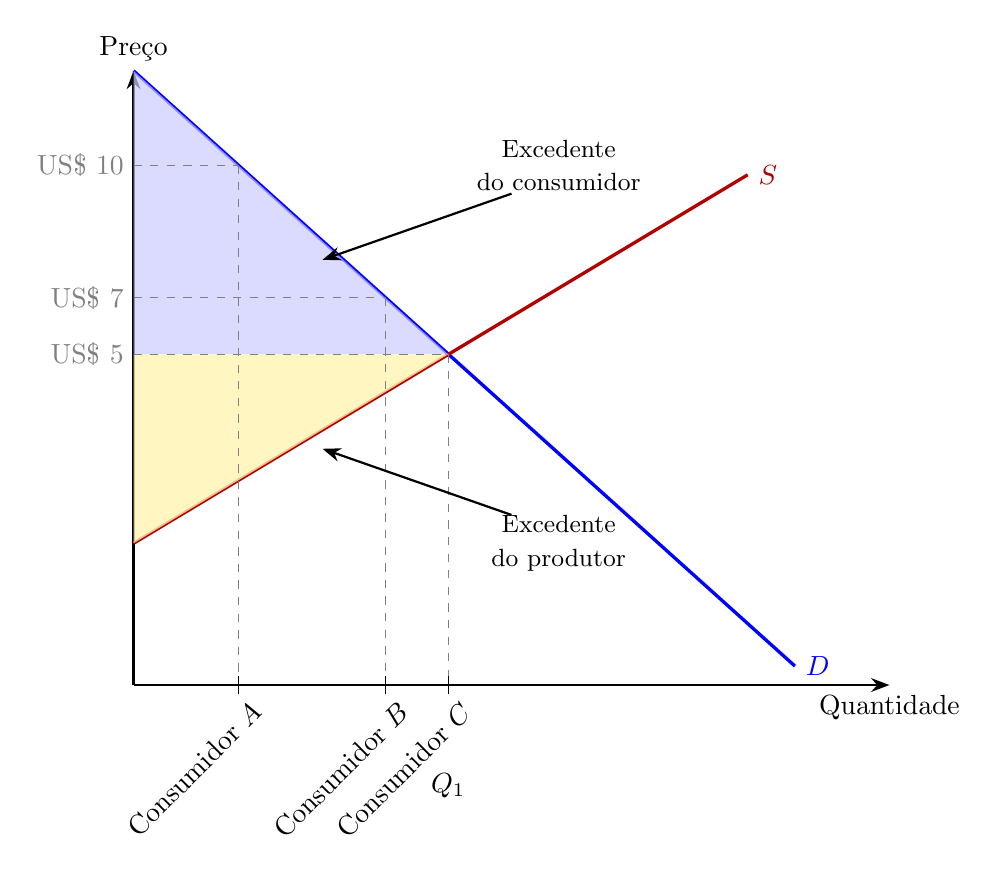
\begin{tikzpicture}[scale=1.2, >=Stealth]
    
    % Eixos
    \draw[thick,->] (0,0) -- (8,0) node[below] {Quantidade};
    \draw[thick,->] (0,0) -- (0,6.5) node[above] {Preço};
    
    % Curvas de oferta e demanda
    \draw[blue, very thick, domain=0:7] plot (\x, {6.5 - 0.9*\x}) node[right] {$D$};
    \draw[red!70!black, very thick, domain=0:6.5] plot (\x, {1.5 + 0.6*\x}) node[right] {$S$};
    
    % Ponto de equilíbrio
    \coordinate (E) at (3.33, 3.5);
    
    % Excedente do consumidor (área azul claro)
    \fill[blue!20, opacity=0.7] (0,6.5) -- (0,3.5) -- (3.33,3.5) -- cycle;
    
    % Excedente do produtor (área bege)
    \fill[orange!30!yellow!30, opacity=0.8] (0,1.5) -- (0,3.5) -- (3.33,3.5) -- cycle;
    
    % Linhas tracejadas horizontais (tocando as curvas)
    \draw[dashed, gray] (0,5.5) node[left] {US\$ 10} -- (1.11,5.5);
    \draw[dashed, gray] (1.11,5.5) -- (1.11,0);
    \draw[dashed, gray] (0,4.1) node[left] {US\$ 7} -- (2.67,4.1);
    \draw[dashed, gray] (2.67,4.1) -- (2.67,0);
    \draw[dashed, gray] (0,3.5) node[left] {US\$ 5} -- (3.33,3.5);
    \draw[dashed, gray] (3.33,3.5) -- (3.33,0);
    
    % Marcações no eixo x
    \draw (1.11,-0.1) -- (1.11,0.1) node[below, rotate=45, anchor=north east, yshift=-2mm] {Consumidor $A$};
    \draw (2.67,-0.1) -- (2.67,0.1) node[below, rotate=45, anchor=north east, yshift=-2mm] {Consumidor $B$};
    \draw (3.33,-0.1) -- (3.33,0.1) node[below, rotate=45, anchor=north east, yshift=-2mm] {Consumidor $C$};
    \draw (3.33,0) node[below, yshift=-10mm] {$Q_1$};
    
    % Rótulos dos excedentes
    \node[align=center] at (4.5, 5.5) {\small Excedente\\\small do consumidor};
    \node[align=center] at (4.5, 1.5) {\small Excedente\\\small do produtor};
    
    % Setas apontando para as áreas
    \draw[->, thick] (4.0, 5.2) -- (2.0, 4.5);
    \draw[->, thick] (4.0, 1.8) -- (2.0, 2.5);
    
\end{tikzpicture}

\end{document}
